% !TEX root = ../main.tex

\chapter{相关研究工作与关键技术基础}

\section{异常检测方法研究现状}

异常检测的目标是在大量正常样本中识别出少量偏离总体分布的对象，其研究长期围绕距离型、密度型、统计型、集成型以及深度学习型方法展开\citep{aggarwal2017outlier,zhao2022tod}。对于金融场景而言，异常对象既可能表现为单笔交易的数值偏离，也可能体现为账户行为、设备特征、时序模式或多实体交互关系中的结构性异常。因此，金融异常检测不仅要求方法具有一定的识别能力和可解释性，还要求其能够在高吞吐、低时延和大规模数据条件下保持可执行性。本文后续所关注的，并非“哪一类方法在理论上最强”，而是“哪一类方法在系统层面更容易被组织为可部署、可扩展的检测链路”。如图~\ref{fig:ad-taxonomy}所示，异常检测方法可以从建模对象和评分机制两个维度进行归类；表~\ref{tab:ad-complexity}进一步比较了各类代表方法在复杂度、可解释性以及大规模金融场景适配性上的差异。

距离型方法是金融异常检测中最常见的一类路线，其基本思想是根据样本与近邻之间的距离、局部连通结构或几何关系来刻画异常程度\citep{aggarwal2017outlier,angiulli2002fast}。例如，基于 $k$ 近邻的异常检测通常将样本与其第 $k$ 个近邻的距离、平均近邻距离或邻域集合结构作为风险评分依据；ABOD、COF、LOF 等方法则进一步引入角度、可达距离或局部密度等信息，以提高对复杂异常模式的识别能力。该类方法的优势在于业务解释直观，与金融风控中“异常样本偏离正常交易模式”的经验认知较为一致。然而，距离型方法通常需要显式或隐式地处理大规模近邻关系，其时间与空间复杂度在朴素实现下往往较高。TOD 对表格型异常检测算法的整理表明，多种 proximity-based 方法在朴素实现下至少具有二次时间或空间复杂度，这直接限制了其在近实时金融场景中的可部署性\citep{zhao2022tod}。

与距离型方法相比，密度型和统计型方法更强调样本在局部分布或全局分布中的稀有程度。密度型方法通常通过比较样本局部密度与邻域密度之间的差异来识别异常，典型代表包括 LOF、LOCI 等；统计型方法则通过特征分布、边缘概率或直方图结构来评估异常程度，例如 HBOS、COPOD 与 ECOD 等\citep{zhao2022tod,breunig2000lof}。这类方法在部分低维或中等维度表格数据上具有较好的效率优势，也更容易与批处理统计过程结合。但从系统实现角度看，密度型方法往往仍然依赖近邻结构，统计型方法则对数据预处理、分布表达和批量组织方式较为敏感，因此其大规模效率并不只由算法公式决定，还强烈依赖底层数据路径与计算资源组织方式。

集成型方法与深度学习型方法则分别代表了两种不同的提升方向。前者通过组合多个检测器或多个子空间模型来提高稳健性，后者则利用深层表征能力处理更复杂的数据分布和非线性模式\citep{aggarwal2017outlier,zhao2022tod}。但对于本文关注的金融大规模异常检测系统而言，这两类方法并不天然占优：一方面，集成方法通常会进一步提高推理成本和系统复杂度；另一方面，深度模型虽然表达能力更强，却往往伴随更高的在线部署成本、更复杂的训练依赖以及较弱的业务可解释性。因此，本文不以提出新的异常检测模型为主要目标，而是更关注如何在保持合理检测效果的前提下，选择\textbf{可解释、可张量化、可分阶段执行}的方法作为评分主干，并通过候选召回与系统优化降低整体检测成本。基于这一判断，本文后续采用“候选召回 + 张量化异常评分”的两阶段系统路线，而不是直接追求更复杂的端到端检测模型。

\begin{figure}[htbp]
  \centering
  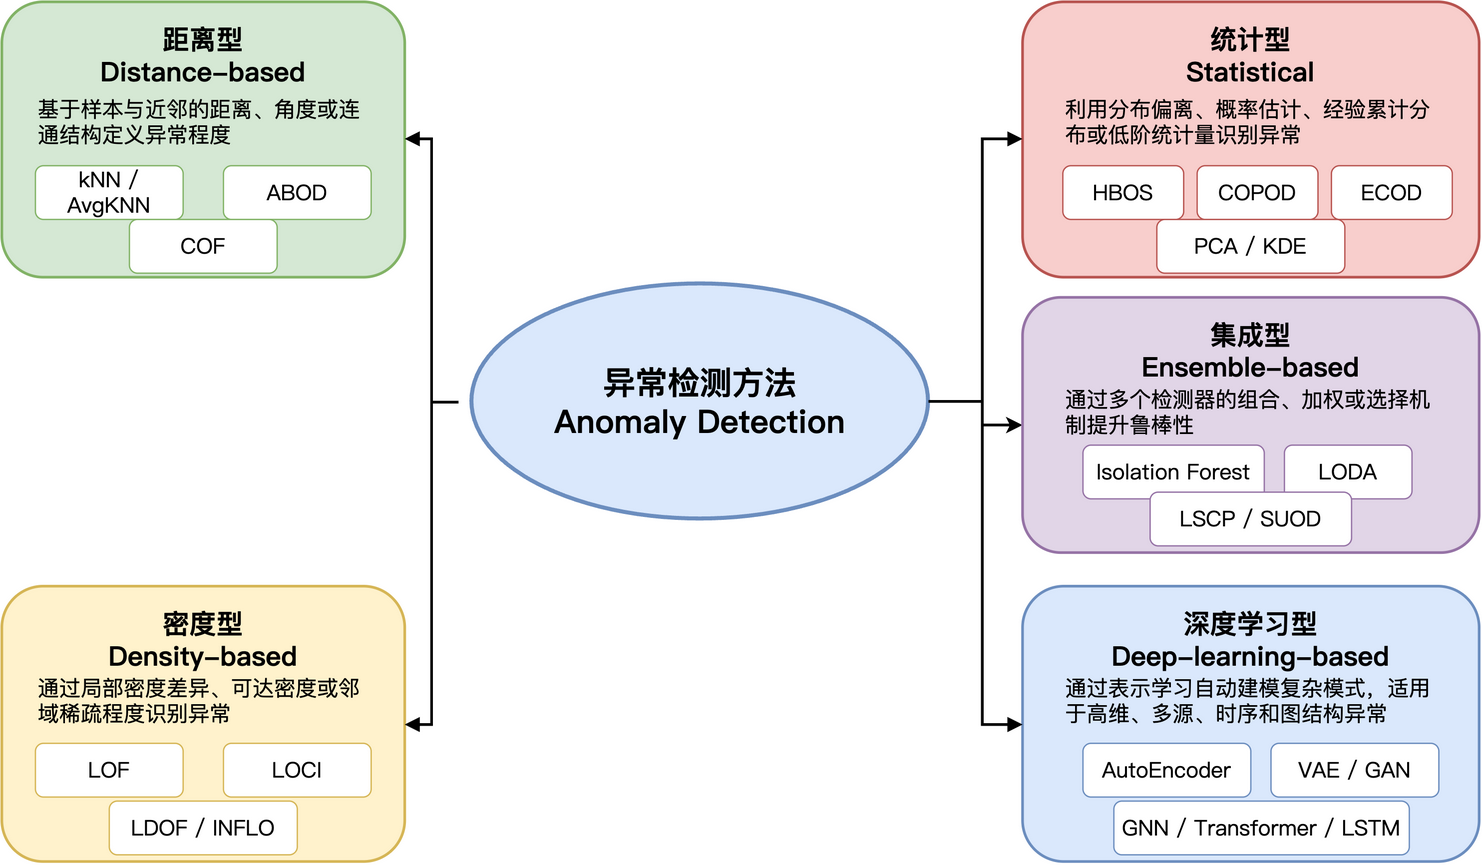
\includegraphics[width=\linewidth]{figures/fig2_1_anomaly_detection_taxonomy.drawio.png}
  \caption{异常检测方法分类图}
  \label{fig:ad-taxonomy}
\end{figure}

\begin{table}[htbp]
  \caption{各类异常检测方法复杂度与系统适配性比较}
  \label{tab:ad-complexity}
  \centering
  \footnotesize
  \setlength{\tabcolsep}{3pt}
  \renewcommand{\arraystretch}{1.25}
  \begin{tabularx}{\linewidth}{@{}p{1.65cm}p{2.55cm}>{\raggedright\arraybackslash}X p{1.7cm}>{\raggedright\arraybackslash}X@{}}
    \toprule
    \textbf{方法类别} & \textbf{代表方法} & \textbf{复杂度与系统特征} & \textbf{可解释性} & \textbf{大规模金融场景适配性} \\
    \midrule
    距离型 & $k$NN、ABOD、COF & 依赖近邻搜索与距离计算，朴素实现下时间和空间开销较高 & 强 & 适合作为评分主干，但通常需要候选召回和 GPU 加速共同支撑 \\
    密度型 & LOF、LOCI & 需要局部密度估计与邻域聚合，复杂度随近邻结构迅速上升 & 较强 & 适合描述相对异常，但系统效率仍受近邻组织和数据路径制约 \\
    统计型 & HBOS、COPOD、ECOD & 依赖边缘分布、分位统计或直方图结构，单次评分较轻量 & 中等 & 适合作为基线或辅助评分模块，但对复杂金融异常模式覆盖有限 \\
    集成型 & Feature bagging、Detector ensemble & 通过组合多个检测器提升稳健性，但推理成本和系统复杂度进一步增大 & 中等 & 适合离线分析或稳健性增强，不利于高吞吐近实时链路 \\
    深度学习型 & Autoencoder、GNN、时序模型 & 表达能力强，但训练与部署依赖重，在线解释和维护成本高 & 较弱 & 适合复杂模式建模，但需要更高工程投入，不是本文主路线 \\
    \bottomrule
  \end{tabularx}
\end{table}

\section{TOD/PyTOD 的方法学基础}

为解决传统异常检测算法难以直接迁移到 GPU 并高效扩展的问题，TOD 提出了一种面向异常检测系统的张量化抽象方法，其核心思想不是为每一种检测器分别编写定制化 GPU 实现，而是将异常检测过程分解为一组基础张量算子与功能算子，并在现代深度学习基础设施上统一执行\citep{zhao2022tod}。如图~\ref{fig:tod-overview}所示，TOD 的系统总览可以概括为三层：底层是可由 GPU 高效执行的基础张量算子，中间层是由基础算子组合而成的功能算子，上层则是具体异常检测算法及其组合形式。图~\ref{fig:algo-to-ops}进一步展示了典型异常检测方法到张量算子的映射关系，例如 $k$NN、LOF、COPOD 等算法可被重写为 \texttt{cdist}、\texttt{topk}、聚合与统计运算的组合\citep{zhao2022tod}。这一抽象的直接意义在于：异常评分不再被视为“只能在 CPU 上完成的算法逻辑”，而可以被组织为标准化、可批处理、可并行的 GPU 计算过程。

TOD 的第二个重要贡献在于其面向大规模场景的系统优化机制，包括 provable quantization、automatic batching 以及 multi-GPU support\citep{zhao2022tod}。其中，量化机制通过在满足精度边界的条件下降低部分算子的内存与计算开销，自动批处理则将原本难以放入单卡显存的大规模异常检测计算拆分为可流水执行的小批次，多 GPU 支持则进一步把这些批次分配到多个设备并行执行。TOD 的相关实验表明，在异常检测任务中，GPU 时间往往占总运行时间的绝大部分，而通过算子融合与批处理优化，可以显著减少大规模中间矩阵的物化和搬运开销，从而提升整体效率\citep{zhao2022tod}。这说明，对于本文所关注的大规模金融数据场景，异常评分是否能够被“张量化 + 批处理 + 多 GPU 化”，比单一检测器的理论公式更决定其系统可落地性。

PyTOD 可以看作 TOD 的开源实现与工程化延展，其价值在于把张量化异常检测从论文级概念推进为可复用的软件能力。对本文而言，PyTOD 的意义主要体现在三个方面：第一，它提供了 $k$NN、LOF、HBOS、ABOD 等多类检测器的统一接口，使本文能够在同一评分主干上比较不同检测器的适配性；第二，它继承了 TOD 所强调的张量算子抽象与 GPU 批处理思路，为后续将异常评分嵌入候选召回链路提供了方法学基础；第三，它天然适合作为“评分主干”而非“完整检测系统”，因为其重点在于异常评分的 GPU 化，而不直接覆盖大规模外存候选召回、GPU--SSD 数据路径以及多设备在线调度等更高层系统问题。表~\ref{tab:pytod-boundary}据此总结了 PyTOD 在本文中的能力边界：可直接复用的是张量化评分能力，需要补强的是候选驱动接口、GPU 常驻输出路径以及与外部召回模块的融合方式。

需要强调的是，早期 GPU 异常检测研究多采用“面向特定算法定制加速”的思路，例如针对距离型异常检测或局部离群检测单独设计 CUDA 版本。与之相比，TOD/PyTOD 所代表的路线更适合本文的研究目标：本文并不打算为某一个检测器单独做高度特化优化，而是希望建立一个能够同时兼容候选召回、批处理评分和多 GPU 扩展的统一系统框架。因此，本文后续以 PyTOD 作为异常评分主干，并不是因为它能够独立解决全部系统问题，而是因为它为“评分阶段的 GPU 化与系统化组织”提供了最合适的基础。

\begin{figure}[htbp]
  \centering
  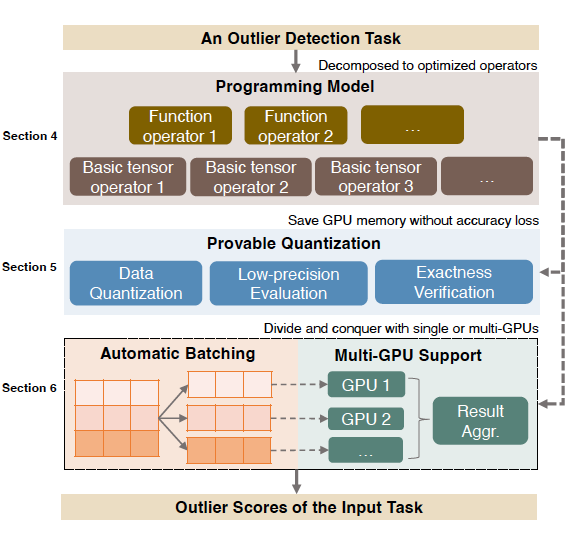
\includegraphics[width=\linewidth]{figures/fig2-2.png}
  \caption{TOD/PyTOD 系统总览图}
  \label{fig:tod-overview}
\end{figure}

\begin{figure}[htbp]
  \centering
  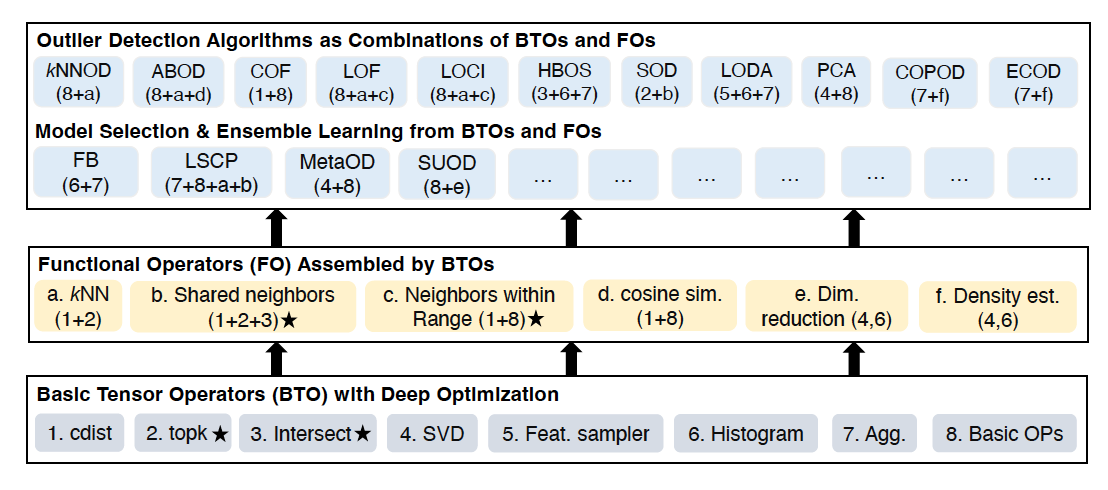
\includegraphics[width=\linewidth]{figures/fig2-3.png}
  \caption{典型异常检测算法到张量算子的映射}
  \label{fig:algo-to-ops}
\end{figure}

\begin{table}[htbp]
  \caption{PyTOD 在本文中的能力边界}
  \label{tab:pytod-boundary}
  \centering
  \footnotesize
  \setlength{\tabcolsep}{3pt}
  \renewcommand{\arraystretch}{1.25}
  \begin{tabularx}{\linewidth}{@{}p{1.9cm}>{\raggedright\arraybackslash}X>{\raggedright\arraybackslash}X>{\raggedright\arraybackslash}X@{}}
    \toprule
    \textbf{能力类别} & \textbf{PyTOD 已支持 / 可直接复用内容} & \textbf{本文未直接覆盖的能力边界} & \textbf{本文中的补强方式} \\
    \midrule
    方法学抽象 & 将异常检测算法抽象为 \textbf{BTOs + FOs}，支持将多种经典 OD 方法映射到 GPU 张量执行语义 & 不负责候选召回与两阶段检索--评分协同 & 由 \textbf{FlashANNS} 提供候选召回，PyTOD 只承担异常评分主干 \\
    异常评分执行 & 支持 $k$NN、LOF、HBOS、COPOD、ECOD、PCA 等多类 OD 算法的 GPU 化评分 & 不直接处理金融业务场景下的多阶段风险检测流水 & 在第三章中将 PyTOD 嵌入到融合检测模型，作为评分后端 \\
    算子层优化 & 支持 \textbf{provable quantization}、operator abstraction、部分 operator fusion 思路 & 不覆盖候选集组织、重排序与 ANN 检索路径管理 & 由本文融合层补充候选集输入组织与评分接口适配 \\
    大规模执行 & 支持 \textbf{automatic batching}，缓解显存不足问题；支持 \textbf{multi-GPU support} & 不解决 SSD-resident 索引、异步 I/O、检索--计算重叠 & 由 FlashANNS 提供 out-of-core 检索与 I/O--compute overlap \\
    系统角色 & 适合作为 \textbf{评分主干}，提供统一、可复用、可 GPU 化的异常评分框架 & 不是完整金融异常检测系统，不包含数据接入、召回、告警与复核闭环 & 本文在第三、四、五章中补足系统融合、数据路径优化和多 GPU 扩展 \\
    工程部署 & 基于 PyTorch，具备较好可扩展性，便于复用现有 GPU 张量基础设施 & 不直接提供面向金融风控在线系统的端到端部署结构 & 本文结合 RAPIDS、FAISS-GPU、FlashANNS 与调度层进行工程化整合 \\
    \bottomrule
  \end{tabularx}
\end{table}

\section{FlashANNS 与候选召回系统}

在大规模异常检测系统中，若直接对全量样本执行精细异常评分，系统往往会因近邻搜索、候选组织和内存占用过大而难以满足吞吐要求。因此，引入高吞吐候选召回模块，以先筛选潜在相关样本、再执行精细评分，是构建近实时检测系统的常见路线。FlashANNS 正是面向这一问题的代表性工作，其核心关注点不是单纯“如何找近邻”，而是“在外存条件下如何使近邻检索中的 I/O 与计算协同推进，从而打破存储—计算瓶颈”\citep{xiao2025flashanns}。如图~\ref{fig:flashanns-io-pipeline}所示，FlashANNS 的基本思想可以概括为异步 I/O---计算流水线：在保持 GPU 计算持续进行的同时，将外存访问与候选扩展过程重叠执行，以减少传统 ANN 图搜索中“先读后算”的严格串行开销。

具体而言，FlashANNS 针对 out-of-core ANN 场景强调三个方面的设计。首先，它通过依赖放松的异步流水线，使部分计算不必等待全部 I/O 完成后再启动，从而提高 GPU 的忙碌度；其次，它利用 warp 级并发和细粒度任务组织提升设备侧对候选扩展与结果筛选的执行效率；再次，它把系统瓶颈从单纯的“计算速度”扩展为“存储路径与计算资源的协同平衡”，强调 ANN 检索在大规模场景下是一个\textbf{I/O---计算联合优化问题}而非单纯算子优化问题\citep{xiao2025flashanns}。从这个意义上看，FlashANNS 与本文的关系不是“替代异常检测”，而是承担候选召回前端，为后续更昂贵的异常评分缩小搜索空间。图~\ref{fig:flashanns-position}展示了 FlashANNS 在本文系统中的位置：它位于候选召回阶段，并与后续 PyTOD 评分阶段构成两阶段融合链路。

从候选召回系统的研究脉络看，传统 ANN 组件、GPU 内存内 ANN 检索和 out-of-core ANN 系统各自关注的瓶颈并不相同。前者更关注索引结构与搜索精度，后者强调设备内向量搜索效率，而 out-of-core 系统则必须额外解决 SSD 访问、对齐 I/O、异步完成信号和大规模索引布局等问题。与一般的内存内 ANN 路线相比，FlashANNS 更适合被放在本文的大规模金融数据背景下讨论，因为本文所面临的问题并不是“单卡内存足够时如何做到最快”，而是在索引规模增大、候选池变大、设备数增加时，如何保持系统整体吞吐不被存储路径拖垮。表~\ref{tab:recall-systems}将传统 ANN 组件、out-of-core ANN 系统与 FlashANNS 的主要特征进行了对比，重点突出它们在 I/O---计算重叠、大规模外存适配性以及与本文系统关系上的差异。

需要指出的是，FlashANNS 解决的是“大规模候选召回”的问题，而不是“异常评分”的问题。它可以显著减轻评分阶段面对的全量搜索压力，但并不直接给出异常分数，也不自动解决后续评分过程中的 GPU 常驻执行、张量组织、候选到评分的接口契约等问题。因此，本文并不将 FlashANNS 视为完整异常检测系统，而是将其与 PyTOD 组合：前者负责高吞吐候选召回，后者负责张量化异常评分。正是这种角色分工，使本文的两阶段系统既继承了 GPU 异常评分的计算优势，也继承了大规模 ANN 检索在外存条件下的吞吐优势。

\begin{figure}[htbp]
  \centering
  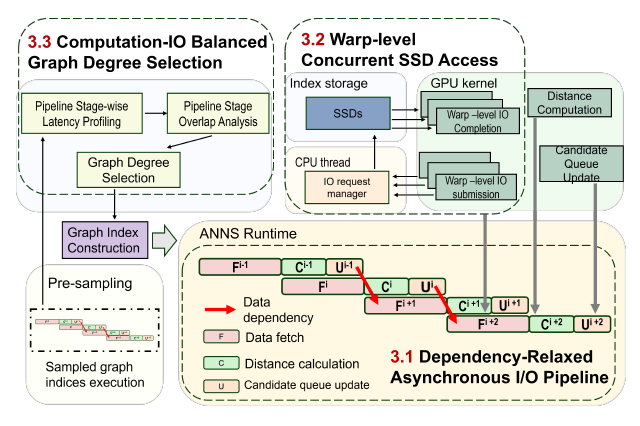
\includegraphics[width=\linewidth]{figures/fig2-4.png}
  \caption{FlashANNS 异步 I/O---计算流水线原理}
  \label{fig:flashanns-io-pipeline}
\end{figure}

\begin{figure}[htbp]
  \centering
  \thesisplaceholderbox{正式版补齐图~2-5}
  \caption{FlashANNS 在本文系统中的位置}
  \label{fig:flashanns-position}
\end{figure}

\begin{table}[htbp]
  \caption{候选召回系统比较}
  \label{tab:recall-systems}
  \centering
  \footnotesize
  \setlength{\tabcolsep}{3pt}
  \renewcommand{\arraystretch}{1.25}
  \begin{tabularx}{\linewidth}{@{}p{2.1cm}p{2.6cm}>{\raggedright\arraybackslash}X p{2.6cm}p{2.4cm}>{\raggedright\arraybackslash}X@{}}
    \toprule
    \textbf{类别} & \textbf{代表方案} & \textbf{主要存储假设} & \textbf{是否考虑 I/O--计算重叠} & \textbf{是否适合大规模外存} & \textbf{主要特点} \\
    \midrule
    传统 ANN 组件 & FAISS、HNSW、IVF/IVF-PQ 等 & 以内存内索引为主，通常假设索引或主要检索结构可驻留内存/显存 & 通常不重点考虑 & 一般较弱 & 检索延迟低、工程成熟、适合中等规模向量召回；但面对超大规模数据时易受内存/显存容量约束 \\
    out-of-core ANN 系统 & SPANN、DiskANN、FusionANNS 等 & 面向 SSD/外存驻留索引，通过磁盘存储支撑更大规模数据 & 部分考虑，但多未充分实现端到端重叠 & 较强 & 能突破内存容量限制，支持更大规模检索；但仍可能存在粗粒度候选过多、CPU 供数瓶颈和 I/O 串行化问题 \\
    FlashANNS & FlashANNS & 明确面向 \textbf{GPU + SSD} 的 out-of-core 图索引检索 & \textbf{是} & \textbf{强} & 通过 dependency-relaxed asynchronous pipeline、warp-level concurrent SSD access 与 computation--I/O balanced graph degree selection 实现高吞吐候选召回 \\
    \bottomrule
  \end{tabularx}
\end{table}

\section{RAPIDS、FAISS-GPU 与工程可部署性}

如果仅从算法流程出发，PyTOD--FlashANNS 融合系统似乎已经能够完成“候选召回---异常评分”两阶段任务；但从工程实现角度看，系统中仍包含大量与算法无关但对性能影响极大的环节，例如金融表格数据预处理、特征整理、批量统计、中间结果表达、向量检索接口组织以及 GPU 内存资源管理等。为此，本文引入 RAPIDS 与 FAISS-GPU 作为系统后端增强组件，以降低这些环节的实现复杂度，并尽可能让关键数据路径保持在 GPU 侧\citep{rapids_cudf_pandas,rapids_rmm_pinned,faiss_gpu_wiki,johnson2019faiss}。如图~\ref{fig:rapids-position}所示，RAPIDS 在本文系统中的作用主要体现在“数据处理路径增强”上；如图~\ref{fig:faiss-interop}所示，FAISS-GPU 则更多承担“设备侧向量检索与互操作能力增强”的职责。表~\ref{tab:rapids-faiss-roles}总结了二者在本文中的功能分工。

RAPIDS 的核心价值在于为 GPU 上的表格处理和数据科学工作流提供统一支持。cuDF 作为其重要组成部分，可以视为面向 GPU 的 DataFrame 引擎，适合处理金融场景中大量以表格形式存在的交易记录、账户属性、设备特征与时间统计结果。对本文而言，RAPIDS 并不承担异常检测本身，而主要承担候选召回前后的数据组织任务，包括字段清洗、特征拼接、归一化、窗口统计、中间结果重排和批量结果合并等。如果这些操作长期停留在 CPU 侧，即便候选召回和异常评分本身已经 GPU 化，系统整体也会因频繁的 CPU$\leftrightarrow$GPU 往返而失去吞吐优势。因此，RAPIDS 的真正意义在于压缩“前处理---候选召回---评分---后处理”之间的数据路径长度，为后续单卡 GPU 主导执行链路奠定基础。

与此同时，RAPIDS 并不意味着“只要用了 GPU DataFrame，整条链路就天然保持在 GPU 上”。在兼容模式或未覆盖操作出现时，部分数据处理流程可能退回 CPU 执行；一旦这种回退发生，系统就会重新引入额外的数据搬运与同步等待。由此可见，RAPIDS 的价值不应被简单理解为“自动加速”，而应被理解为“为构建统一 GPU 数据路径提供可能性，但仍需结合具体算子覆盖范围与运行路径进行约束”。这也意味着，本文后续在第四章讨论数据路径优化时，必须把“哪些处理确实保留在 GPU、哪些处理可能回退到 CPU”作为工程边界显式说明，而不能把名义上的 GPU 化直接等同于真实执行链路中的 GPU 常驻。

FAISS-GPU 的价值则更多体现在设备侧向量检索能力和 GPU 资源组织能力两个方面。作为成熟的向量检索后端，FAISS-GPU 支持在 GPU 上完成向量索引构建、近邻检索和部分结果筛选，其 \texttt{StandardGpuResources} 通过预分配 scratch memory 与 CUDA stream 组织方式，能够减少频繁 \texttt{cudaMalloc/cudaFree} 带来的同步与抖动\citep{faiss_gpu_wiki,johnson2019faiss}。此外，FAISS-GPU 还明确区分 host pointer 输入和 device pointer 输入两类路径：若输入已经位于同一 GPU 上，则可以避免额外拷贝；若输入位于主机端或位于不同设备上，则会引入相应的数据搬运开销。正因如此，FAISS-GPU 在本文中的作用不仅是“提供一个能跑的向量检索后端”，更重要的是为后续分析 CPU/GPU 互操作路径、解释何处发生额外拷贝以及设计 GPU 常驻数据路径提供工程依据。

从角色分工上看，RAPIDS 与 FAISS-GPU 分别服务于“数据处理路径”和“向量检索路径”。前者让金融表格型数据及中间结果组织尽量留在 GPU；后者为候选检索提供高性能设备侧实现与成熟资源管理。二者的共同目标是压缩 CPU 与 GPU 之间的非必要往返，使 PyTOD--FlashANNS 融合系统不止在候选召回和异常评分两个单点上更快，而是在整条执行链路上更低开销、更可部署。也正因如此，本文在后续章节中不会把 RAPIDS 与 FAISS-GPU 当作“额外附属工具”，而是把它们视为构建 GPU 主导端到端执行链路的工程支撑组件。

\begin{figure}[htbp]
  \centering
  \thesisplaceholderbox{正式版补齐图~2-6}
  \caption{RAPIDS 在本文系统中的数据处理位置}
  \label{fig:rapids-position}
\end{figure}

\begin{figure}[htbp]
  \centering
  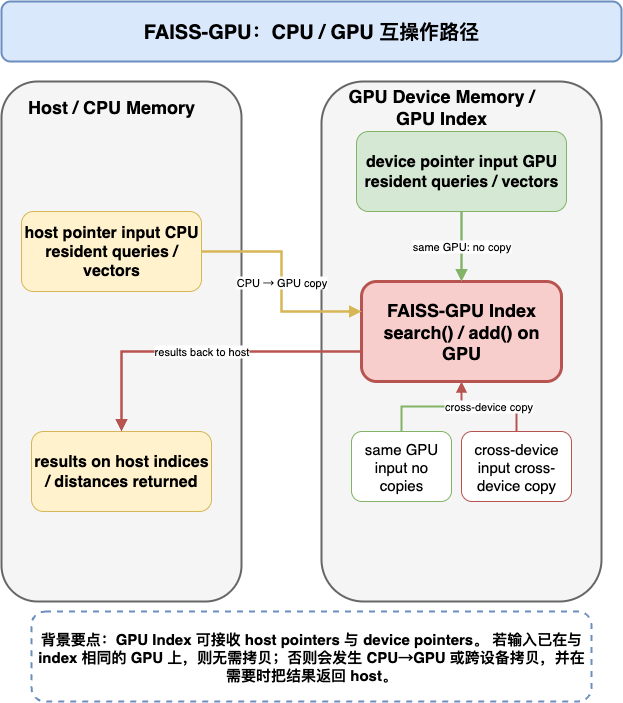
\includegraphics[width=\linewidth]{figures/fig2_6_2_7_rapids_faiss_paths-Page-1.drawio.png}
  \caption{FAISS-GPU 的 CPU/GPU 互操作路径}
  \label{fig:faiss-interop}
\end{figure}

\begin{table}[htbp]
  \caption{RAPIDS 与 FAISS-GPU 的功能分工}
  \label{tab:rapids-faiss-roles}
  \centering
  \footnotesize
  \setlength{\tabcolsep}{3pt}
  \renewcommand{\arraystretch}{1.25}
  \begin{tabularx}{\linewidth}{@{}p{2.0cm}>{\raggedright\arraybackslash}X>{\raggedright\arraybackslash}X>{\raggedright\arraybackslash}X>{\raggedright\arraybackslash}X@{}}
    \toprule
    \textbf{组件} & \textbf{主要功能} & \textbf{在本文系统中的位置} & \textbf{主要收益} & \textbf{能力边界 / 潜在限制} \\
    \midrule
    RAPIDS / cuDF & GPU DataFrame、字段清洗、特征拼接、窗口统计、中间结果重排 & 位于候选召回前后的数据处理路径 & 缩短 CPU$\leftrightarrow$GPU 往返，提升表格型数据处理吞吐 & 若走兼容模式或未覆盖算子，可能发生 CPU fallback \\
    RAPIDS / RMM & 内存池、页锁定主机内存、设备与主机资源管理 & 位于关键数据交换与缓冲区管理层 & 降低频繁分配释放带来的抖动，提升必要边界传输稳定性 & 不能替代链路设计本身，仍需控制数据交换边界 \\
    FAISS-GPU & GPU 侧索引构建、近邻检索、资源对象与 stream 管理 & 位于候选召回与设备侧向量检索路径 & 提供成熟高性能检索后端，减少额外拷贝与资源抖动 & host/device/cross-device 路径代价不同，若接口组织不当仍会引入数据搬运 \\
    \bottomrule
  \end{tabularx}
\end{table}

\section{多 GPU 调度与在线推理启示}

当单卡系统的吞吐率接近上限，或单卡显存无法容纳更大索引与更大批次时，多 GPU 扩展便成为提升系统能力的自然方向。然而，多 GPU 并不意味着性能一定线性增加，因为更多 GPU 同时也意味着更复杂的查询分发、索引组织、设备间通信、结果归并和共享 I/O 竞争。TOD 的多 GPU 支持已经说明，批处理任务可以被分配到多个设备并行执行，从而在算子级别提升总体吞吐\citep{zhao2022tod}；但对于本文所关注的“候选召回 + 异常评分”两阶段系统而言，多 GPU 扩展不仅是“多做一点同样的计算”，而是需要在候选召回、评分、归并和 I/O 之间重新组织数据路径和控制路径。图~\ref{fig:rep-vs-shard}对比了 replicated 与 sharded 两类多 GPU 扩展模式，图~\ref{fig:cpu-vs-gpu-merge}展示了 CPU 聚合与 GPU 侧归并两种路径的差异，表~\ref{tab:multi-gpu-strategies}进一步总结了这些策略的适用条件与系统代价。

从扩展策略看，replicated 与 sharded 分别对应两种不同的设计哲学。replicated 模式倾向于在每张 GPU 上保留完整索引或完整功能链路，使每个设备可以独立完成本地候选召回和异常评分；其优点在于查询路径简单、设备间协同较少，更适合吞吐优先的在线推理场景。sharded 模式则通过在多设备间分片索引或数据来扩展容量，能够支持更大规模索引，但也会引入额外的跨设备归并与同步开销。对本文而言，replicated 更符合金融近实时检测场景的目标：单次请求的关键是稳定吞吐和低尾延迟，而不是极限压缩单卡显存占用。因此，后续多 GPU 主线优先考虑 replicated 架构；当容量约束使得跨卡归并不可避免时，再进一步讨论 sharded 及其归并代价\citep{cuvs_multi_gpu_nn,cuvs_multi_gpu_ivf_host}。

在归并路径上，CPU 聚合与 GPU 侧归并的差异尤为关键。若多个设备在本地生成候选或分数后，统一回到 CPU 做聚合，则虽然实现简单，但会把 CPU 重新拉回数据平面，进而造成额外的 D2H/H2D 搬运和同步等待。相反，如果将跨卡归并逻辑尽量下沉到 GPU，并结合 NCCL 等设备间通信机制，则可以把更多中间结果留在设备侧，减少主机聚合带来的瓶颈。NCCL 官方文档指出，其集体通信操作会异步入队到指定 CUDA stream 上执行，但在同一 \texttt{ncclGroupStart/End()} 组内混用多个 stream 会形成所有 stream 之间的全局同步点\citep{nccl_stream_semantics}。这说明 GPU 侧归并虽优于 CPU 聚合，但如果通信流和计算流组织不当，也可能引入新的同步开销。

除了设备间通信，存储路径与硬件拓扑同样会限制多 GPU 扩展上限。无论采用外存候选召回，还是采用多设备共享存储路径，GPU---SSD---PCIe---NUMA 之间的拓扑关系都可能使“理论上的并行收益”无法在实际系统中完全实现。共享 PCIe 交换机、共享 SSD 通道或非对称 NUMA 路径，都可能使部分设备在高并发下遭遇 I/O 争用，从而把瓶颈重新转移到存储子系统。GPUDirect Storage 文档指出，如果 GPU、NIC 与存储设备位于更理想的 PCIe 拓扑关系下，可以减少 CPU bounce buffer 并提升带宽利用效率\citep{gds_overview,gds_design_guide}。这意味着，多 GPU 扩展不能只看 GPU 之间的负载均衡，还必须考虑拓扑感知 I/O lane 绑定、准入控制以及共享路径下的资源组织策略。

综合而言，现有多 GPU 调度与在线推理研究为本文提供了三点启示：其一，在吞吐优先的金融异常检测场景下，应优先采用 replicated 架构，让每张 GPU 尽量独立完成候选召回与异常评分；其二，当必须跨卡归并时，应尽量将归并逻辑下沉到 GPU 并利用 NCCL 通信，而不是回到 CPU 聚合；其三，多 GPU 扩展的上限不仅受设备数目影响，也受制于存储路径、PCIe/NUMA 拓扑与 I/O 资源组织方式。因此，本文后续的多 GPU 设计不是单纯“加更多 GPU”，而是围绕“CPU 控制面 + GPU 数据平面 + 拓扑感知 I/O 控制”构建完整扩展路径。

\begin{figure}[htbp]
  \centering
  \thesisplaceholderbox{正式版补齐图~2-8}
  \caption{replicated 与 sharded 两类多 GPU 扩展模式对比}
  \label{fig:rep-vs-shard}
\end{figure}

\begin{figure}[htbp]
  \centering
  \thesisplaceholderbox{正式版补齐图~2-9}
  \caption{CPU 聚合路径与 GPU 侧归并路径对比}
  \label{fig:cpu-vs-gpu-merge}
\end{figure}

\begin{table}[htbp]
  \caption{多 GPU 扩展策略比较}
  \label{tab:multi-gpu-strategies}
  \centering
  \footnotesize
  \setlength{\tabcolsep}{3pt}
  \renewcommand{\arraystretch}{1.25}
  \begin{tabularx}{\linewidth}{@{}p{2.0cm}>{\raggedright\arraybackslash}X>{\raggedright\arraybackslash}X>{\raggedright\arraybackslash}X>{\raggedright\arraybackslash}X@{}}
    \toprule
    \textbf{策略} & \textbf{核心思路} & \textbf{优势} & \textbf{代价 / 风险} & \textbf{本文中的定位} \\
    \midrule
    Replicated & 每张 GPU 持有完整索引与完整执行链路，查询在设备间分发 & 查询路径简单，跨卡协同少，吞吐扩展更直接 & 需要更多显存，索引复制成本较高 & 多 GPU 主方案，适合吞吐优先金融场景 \\
    Sharded & 多张 GPU 分片保存索引或数据，单次查询需跨卡协同 & 可支持更大容量，降低单卡显存压力 & 需要跨卡归并与更复杂同步，尾延迟更敏感 & 容量受限时的兜底路径 \\
    CPU 聚合 & 各 GPU 输出局部结果后统一回 CPU 归并 & 实现相对简单，工程门槛较低 & CPU 重回数据平面，D2H/H2D 往返和同步开销高 & 不作为主方案，仅用于对比和边界分析 \\
    GPU 侧归并 & 在设备侧完成局部结果合并，并结合 NCCL 通信 & 减少主机聚合瓶颈，中间结果更易留在 GPU 上 & 通信流组织不当时可能形成新的同步点 & sharded 或特殊约束场景下优先采用 \\
    拓扑感知 I/O 控制 & 结合 PCIe/NUMA/SSD 拓扑进行 lane 绑定与准入控制 & 降低共享存储路径争用，更接近真实扩展收益 & 需要硬件拓扑感知和额外调度策略 & 多 GPU 上限控制的重要配套机制 \\
    \bottomrule
  \end{tabularx}
\end{table}

\section{本章小结}

本章围绕本文研究对象所涉及的关键技术与相关研究进行了系统梳理，并尝试从“本文为何采用这一技术路线”的角度重构相关工作。首先，从异常检测方法角度看，距离型、密度型和统计型方法为金融异常检测提供了理论基础，但在大规模场景下普遍面临复杂度与可扩展性约束，因此单纯比较模型类别并不足以支撑系统设计\citep{aggarwal2017outlier,zhao2022tod}。其次，从 GPU 异常检测系统角度看，TOD/PyTOD 通过张量算子抽象、自动批处理与多 GPU 支持证明了异常评分可以被统一映射到 GPU 执行框架中，从而为本文选取 PyTOD 作为评分主干提供了方法学依据\citep{zhao2022tod}。再次，从候选召回系统角度看，FlashANNS 强调异步 I/O---计算流水线和存储—计算平衡，说明大规模 ANN 检索的关键问题并不只是近邻精度，而是候选召回如何与底层 I/O 路径协同推进\citep{xiao2025flashanns}。同时，RAPIDS 与 FAISS-GPU 分别为 GPU 表格数据处理与 GPU 向量检索提供了成熟后端能力，使构建统一 GPU 数据路径成为可能\citep{rapids_cudf_pandas,faiss_gpu_wiki}。最后，多 GPU 调度与在线推理研究进一步表明，replicated 与 sharded 的选择、GPU 侧归并、NCCL 通信以及拓扑感知 I/O 控制共同决定了多设备场景下的系统扩展能力\citep{cuvs_multi_gpu_nn,nccl_stream_semantics,gds_overview,gds_design_guide}。

通过上述分析可以看出，现有研究已经分别在异常评分、候选召回和多 GPU 扩展等方面提供了较为充分的基础，但尚缺少一个面向金融大规模异常检测任务、能够同时统筹候选召回、异常评分、数据路径优化与多 GPU 扩展的统一系统框架。本文正是在这一空白处切入：以 PyTOD 为异常评分主干，以 FlashANNS 为候选召回模块，并结合 RAPIDS、FAISS-GPU、GPU 常驻执行链路以及多 GPU 数据并行与 GPU 侧归并机制，构建一套可部署、可扩展、可验证的金融异常检测系统。为便于后续章节衔接，表~\ref{tab:chapter2-summary}对本章涉及的相关技术、能力边界及其与本文系统设计的关系进行了归纳。第三章将在此基础上进一步给出 PyTOD--FlashANNS 融合模型、实验数据准备与基础执行流程设计。

\begin{table}[htbp]
  \caption{本章相关技术、能力边界及其与本文系统设计的关系}
  \label{tab:chapter2-summary}
  \centering
  \footnotesize
  \setlength{\tabcolsep}{3pt}
  \renewcommand{\arraystretch}{1.25}
  \begin{tabularx}{\linewidth}{@{}p{2.2cm}>{\raggedright\arraybackslash}X>{\raggedright\arraybackslash}X>{\raggedright\arraybackslash}X@{}}
    \toprule
    \textbf{技术 / 研究方向} & \textbf{已提供能力} & \textbf{能力边界 / 未解决问题} & \textbf{与本文系统设计的关系} \\
    \midrule
    传统异常检测方法 & 提供距离、密度、统计等异常性定义与业务解释基础 & 大规模场景下复杂度高，难以单独支撑近实时系统 & 为本文选择“候选召回 + 张量化评分”路线提供方法学背景 \\
    TOD / PyTOD & 提供张量算子抽象、GPU 评分、自动批处理与多 GPU 评分基础 & 不直接覆盖大规模候选召回、外存索引与端到端系统调度 & 作为本文异常评分主干与 GPU 评分骨架 \\
    FlashANNS & 提供 out-of-core ANN 检索、异步 I/O---计算流水线和高吞吐候选召回能力 & 不直接输出异常分数，也不自动解决后续评分接口与数据路径问题 & 作为本文候选召回前端，与 PyTOD 形成两阶段链路 \\
    RAPIDS & 提供 GPU DataFrame、数据清洗、统计处理和内存资源管理能力 & 若使用不当仍可能回退 CPU，不能替代链路级优化 & 作为数据处理路径增强组件，支撑 GPU 主导执行链路 \\
    FAISS-GPU & 提供成熟的设备侧向量检索、资源对象与 host/device 互操作机制 & 不同输入路径代价不同，若接口组织不当仍会引入拷贝 & 作为候选检索后端增强组件，支撑设备侧连续执行 \\
    多 GPU 调度与在线推理研究 & 提供 replicated / sharded、设备通信与拓扑优化等经验 & 需要结合具体数据路径和存储拓扑做系统化落地 & 为第五章的数据并行、GPU 侧归并和 I/O 控制提供设计依据 \\
    \bottomrule
  \end{tabularx}
\end{table}
